\pdfminorversion=4

\documentclass[a4paper,english,twocolumn]{article}

\usepackage[utf8]{inputenc}
\usepackage{ae,aecompl,url,natbib,graphicx}
\usepackage[english]{babel}

\parskip 1ex
\parindent 0pt
\evensidemargin 0mm
\oddsidemargin 0mm
\textwidth 159.2mm
\topmargin 0mm
\headheight 0mm
\headsep 0mm
\textheight 246.2mm

\pagestyle{plain}

\bibpunct{(}{)}{;}{a}{,}{,}

\newcommand*\rot{\rotatebox{90}}

% ---------------------------------------------------------------------

\begin{document}

\title{T-111.5360 Report: Remote Mouse}

\author{Valter Kraemer, valter.kraemer@aalto.fi\\Ville Skyttä, ville.skytta@iki.fi\\Aalto University}

\date{\today}

\maketitle

% ---------------------------------------------------------------------

\section{Introduction}

WebSockets is a technology providing an efficient full-duplex
bidirectional communications channel between clients and servers. Due
to its low latency characteristics, it is well suited for real time
applications. The WebSocket protocol is standardized by IETF
\citep{rfc} and W3C \citep{w3c} develops an API to enable its use in
web pages.

In this report we introduce Remote Mouse, a virtual mouse pointer on a
web page, controlled from another web device. WebSockets is used as
the communications technology between the devices, through an
intermediate server.

\section{Related work}

\citet{bassbouss} address multi-screen web application development and
the transformation of traditional web applications to multi-screen
capabilities. Both the current and proposed multi-screen application
models utilize WebSocket in communications between clients (screens)
and servers.

Agar.io\footnote{\url{http://agar.io/}} is a massively multiplayer
online game. Players control cells in a petri dish, attempting to grow
larger by consuming pellets and other cells, and avoiding being
consumed by other cells. The game is available for web browsers on its
website, and Android and iOS versions are available for mobile
devices. The web version uses an HTML canvas and its 2D context for
rendering, as well as HTML animation frames. Communication between the
browser and the server is implemented using WebSockets. Data is
transferred using WebSocket binary frames (WebSocket opcode 2), which
are constructed using the ECMAScript 6 ArrayBuffer and DataView
objects. Due to the binary nature of the data, the exact semantics of
it are not available. During gameplay, the traffic consists of on the
order of 50 WebSocket frames per second, with their sizes ranging
approximately from a few to 200 bytes.

YouTube has a feature with which it is possible to control another
YouTube window's video controls from another screen, such as a
computer or a mobile device. It is primarily intended for controlling
YouTube on smart TVs, but can also be used in a browser. The
controlled screen\footnote{\url{http://www.youtube.com/tv}} is
operated by its paired
remote\footnote{\url{http://www.youtube.com/pair}}. The remote works
by sending POST requests to the server that forwards them to the
controlled window. It also uses polling every 10 seconds to check that
the controlled device is still available. The controlled window uses
long polling to check if any information is updated. YouTube is using
LocalStorage for storing information about the playback device and
different identifiers. MediaSource is used to attach sources to their
video elements.

Remot.io\footnote{\url{http://remot.io/}} is a service that controls
HTML presentations such as
reveal.js\footnote{\url{http://lab.hakim.se/reveal-js}} from touch
based devices. The controlling device sends POST requests to the
server that forwards them to the controlled device using long polling
by the controlled device. Remot.io is using touch events for their
remote. Swipe gestures translate to the directions the user wants to
navigate in the slides.

\section{Results}

Using Remote Mouse starts with going to its front page. Devices that
are going to be controlled install a bookmarklet that enables control
by a connected controller. Typically this is carried out by dragging
the bookmarklet into the browser's bookmarks toolbar or
equivalent. The bookmarklet must be installed only once; after that it
can be invoked directly from the bookmarks.

There are three versions of the bookmarklet available. The first two,
heroku and localhost, load the controlling JavaScript code from and
communicate using WebSockets with the respective server, one hosted at
Heroku, or one running locally. The third one, heroku inline, is the
same as the normal Heroku one with the exception that it contains the
entire JavaScript code in the bookmarklet instead of causing it to be
loaded from the server on demand. The inlined code has been minified
using the Google Closure
Compiler\footnote{\url{http://closure-compiler.appspot.com/}}.

When the bookmarklet is invoked, a URL for the controller is
presented. By loading this URL, a session between the controller and
controllee is established and the remote control can start. The URL is
presented also as a QR Code to make it easy to invoke with mobile
devices.

\begin{figure}[htb]
  \begin{center}
    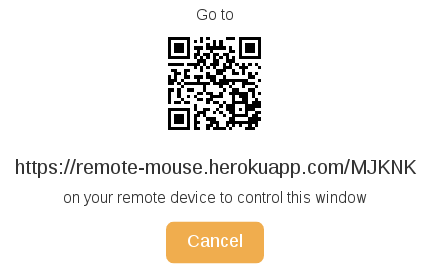
\includegraphics[scale=0.3]{prompt}
    \caption{Controller prompt}
  \end{center}
\end{figure}

When a controller joins the session by loading the session URL, the
popup on the controllee closes and the session starts. A virtual mouse
pointer image is displayed on the controllee, and the controller UI is
shown on the controlling device. Most of the controller window is
empty and serves as the area for mouse and touch movements.

For non-touch devices, the controller document has \verb!mousemove!
and \verb!click!  event handlers. Each mousemove event results in the
pointer position being sent to the server in a WebSocket message. For
touch devices, the document contains event listeners
for \verb!touchstart!, \verb!touchmove!, and
\verb!touchend!.

Positions are sent as pairs of floating point numbers between 0 and 1,
representing the relative left and top position offsets of the event
in percents, proportional to the dimensions of the controller
window. The controllee moves the virtual pointer according to these
values, by converting them to percentages for the virtual pointer's
\verb!left! and \verb!top! CSS properties.

WebSocket messages for click events contain only the information that
the controller requests a click; there is no position information
included with it. The controllee locates the element which is the
target of the click based on its own virtual pointer position, using
the Document.elementFromPoint CSSOM View Module
method\footnote{\url{http://www.w3.org/TR/cssom-view/}}.

Scrolling is implemented in two ways. For touch devices, a two-finger
touch move event translates to scrolling the controllee's view. The
second scroll implementation is done using the DeviceOrientation
API\footnote{\url{http://www.w3.org/TR/orientation-event/}}. Tilting
the controller up and downwards results in scrolling the controllee's
document accordingly. Tilt-scrolling can be toggled on and off with a
three finger touch event.

To aid in analysis and development, the controller contains a debug
bar at the top of the controller window. Display of the debug bar is
toggled from the bottom right corner of the controller UI. It contains
controls for artificially increasing the latency at the server side,
interval how often to send events to the server, how many events to
pack in a single WebSocket payload, sending only every n'th event, as
well as indicator displaying the current measured latency.

\begin{table} \centering
  \begin{tabular}{rl}
    Event & Example message \\
    \hline
    Session request & \verb!create:KJK4B! \\
    Session response & \verb!roomcode:KJK4B! \\
    Position change & \verb!pos:0.7245,0.6241! \\
    Click & \verb!click:left! \\
    Scroll & \verb!scroll:-0.004555! \\
    Latency adjustment & \verb!setLatency:10! \\
    Latency request & \verb!ping:null! \\
    Latency response & \verb!pong! \\
    Controllee not present & \verb!error:noClient! \\
    \hline
  \end{tabular}
  \caption{WebSocket message payloads}
  \label{table:messages}
\end{table}

The server between the controller and controllee is implemented with
Node.js, using the Express\footnote{\url{http://expressjs.com/}} and
ws\footnote{\url{https://github.com/websockets/ws}} modules. The
server is mostly just a relay that forwards messages from controller
to controllee, keeps track of sessions between them and notifies them
about other parties' presence, responds to latency requests, and
implements artificial latency throttling. Express is included only in
order to be able to easily serve static files from the same server as
the WebSockets implementation, otherwise the built-in http module of
Node.js along with ws would suffice.

The application's development is hosted in a GitHub repository located
at \url{https://github.com/valterkraemer/Remote-Mouse}. The server can
be run locally with the command \verb!node app.js! in the project's
top level directory. By default, it listens on port 3000 and can be
accessed at \url{http://localhost:3000/}. Pushes to the GitHub
repository are automatically deployed in the public Heroku instance at
\url{https://remote-mouse.herokuapp.com/}. The Heroku instance uses
the secure \verb!https! and \verb!wss! protocols in order to make it
possible to control web applications served over both \verb!http! and
\verb!https! protocols with it.

The controllee implementation consists of roughly 5 kB of non-minified
JavaScript code (3 kB minified, embeddable to a bookmarklet) which
includes the virtual pointer image as a data URL, and a few hundred
bytes of CSS. The controller side is about 6 kB of non-minified
JavaScript, and 3 kB of HTML and CSS. The server implementation is
about 4 kB JavaScript.

\section{Analysis}

\subsection*{Technology stack}

The most important technology for both controller and controllee sides
of the Remote Mouse implementation is WebSockets. According to
caniuse.com, it is fully supported in all current major browsers since
2013\footnote{\url{http://caniuse.com/#feat=websockets}}. The Node.js
ws library used on the server side has had releases available from
GitHub since
2011\footnote{\url{https://github.com/websockets/ws/releases}}.

The DeviceOrientation API used to implement scrolling based on
controller orientation is also well supported in current browsers to
the extent required by Remote Mouse. According to
caniuse.com\footnote{\url{http://caniuse.com/#feat=deviceorientation}},
only Microsoft Edge has full support for it, most other browsers have
partial support, and the desktop version of Safari has none. Safari's
non-support is not a major problem, because controller devices are
expected to be mobile ones, and the iOS Safari supports the API.

Table~\ref{table:caniuse} summarizes support for WebSockets and
DeviceOrientation in major browsers. The versions listed are the first
ones in which full support for the technology appeared, followed by
the release year in parenthesis. If full support is not yet available,
the version number in parenthesis indicates the first version with
partial support.

\begin{table} \centering
  \begin{tabular}{rcc}
    & \rot{WebSockets} & \rot{Device-}\rot{Orientation} \\
    \hline
    IE & 10 (2012) & (11) (2013) \\
    Edge & 12 (2015) & (12) (2015) \\
    Firefox & 11 (2012) & (6) (2011) \\
    Chrome & 16 (2011) & (7) (2010) \\
    Safari & 7 (2013) & - \\
    iOS Safari & 6.1 (2013) & (4.3) (2011) \\
    Android Browser & 4.4 (2013) & (3) (2011) \\
    Chrome for Android & 47 (2015) & (47) (2015) \\
    \hline
  \end{tabular}
  \caption{caniuse.com: WebSockets and DeviceOrientation support in selected browsers}
  \label{table:caniuse}
\end{table}

Other browser side technologies besides these two used in Remote Mouse
are basic ones that can nowadays be assumed to be present in
practically all browsers.

\subsection*{User experience}

To test the subjective effect of latency on user experience, a test
with three users was conducted. The users were first asked to use an
Apple Magic
Trackpad\footnote{\url{https://en.wikipedia.org/wiki/Magic_Trackpad}}
to get a feeling of a local, low latency user experience. Then, they
were asked to use Remote Mouse with the latency throttle set to
varying settings. The latency settings were shuffled, i.e. not
presented in increasing or decreasing order in order to avoid users'
expectations affecting the results. Users were tasked to grade the
quality of the pointer control experience in scale from 0 to 10, with
grade 0 being the lowest one, equal to unusable, and 10 being equally
good as the Magic Trackpad.

\begin{table} \centering
  \begin{tabular}{rlrlrl}
    \rot{Latency} & \rot{Grade} & \rot{Latency} & \rot{Grade} & \rot{Latency} & \rot{Grade} \\
    \multicolumn{2}{c}{User 1} & \multicolumn{2}{c}{User 2} & \multicolumn{2}{c}{User 3} \\
    \hline
    500 ms & 2  & 400 ms & 2  & 0 ms   & 8 \\
    200 ms & 4  & 100 ms & 5  & 500 ms & 1 \\
    100 ms & 5  & 300 ms & 4  & 300 ms & 4 \\
      0 ms & 6    & 0 ms & 8  & 100 ms & 8 \\
    100 ms & 6  & 100 ms & 8  & 0 ms   & 9 \\
      0 ms & 8    & 0 ms & 8  & 200 ms & 7 \\
    \hline
  \end{tabular}
  \caption{Subjective user test results}
  \label{table:userresults}
\end{table}

\begin{figure}[htb]
  \begin{center}
    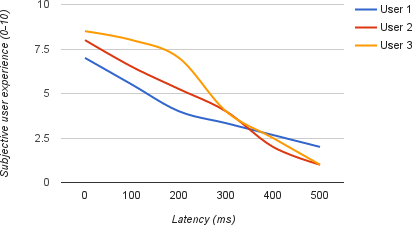
\includegraphics[scale=0.4]{latency}
    \caption{Latency effect on user experience}
    \label{fig:userlatency}
  \end{center}
\end{figure}

All three users rated the experience to belong in the middle of the
scale at approximately 250 ms latency. 500 ms was classified as barely
usable, and 0 to 100 ms quite acceptable. User test data is included
in table~\ref{table:userresults} and visualized in
figure~\ref{fig:userlatency}.

\subsection*{Performance characteristics}

To aid in estimating how these estimates translate to use of Remote
Mouse in different network setups, table~\ref{table:setuplatencies}
lists the typical latencies when the service is running in Heroku and
locally, and when it is being used over different network
connections.

\begin{table} \centering
  \begin{tabular}{rll}
    Network & Server & Latency \\
    \hline
    2G & Heroku    & 500 ms \\
    3G & Heroku    & 70 ms \\
    LTE & Heroku   & 70 ms \\
    Wi-Fi & Heroku & 70 ms \\
    Wi-Fi & local  & 5 ms \\
    \hline
  \end{tabular}
  \caption{Typical setup latencies}
  \label{table:setuplatencies}
\end{table}

Using Google Chrome, running both the controller and controllee in the
same instance of the browser on a Intel Core i7-3610QM 2.30GHz Quad
core laptop running Fedora 23 Linux, and with a local Remote Mouse
server, results in roughly 9\% CPU usage evenly distributed across
cores under rapid pointer movements.

When the pointer is being moved at normal speeds in the above laptop
setup, the Remote Mouse controller sends roughly 80 to 90 WebSocket
messages per second. Moving the pointer faster increases it up to 120
messages per second. Each pointer position message is about 40 bytes
with batch size 1, translating to roughly 5 kB/s bandwidth
requirement. This requirement would however only be achieved if the
WebSocket message size was optimally fitted with the network MTU size
which is rarely if ever the case. Submitting the small message in much
larger frames results in suboptimal use of network bandwidth.

The debug bar's controls allow examination of how various
environmental and optimization aspects affect the user
experience. Decreasing the frequency of sent events decreases network
bandwidth usage but results in choppier pointer movements observed on
the controllee. Bundling several position events into one WebSocket
payload has beneficial networking implications, but without specific
implementation on the controllee, has the same effect as if only the
last of the message's position events was sent. This is because the
controllee browser does not keep up with all CSS positioning events
resulting from the rapid stream of them coming while the payload is
being parsed, but just renders the last of them.

\subsection*{Implementation}

The bookmarklet script approach works without any additional
extensions or plugins installed and thus is very easy to deploy and
invoke. However, the script injection approach has two significant
drawbacks.

First, because the script is injected to the controlled document, it
does not survive page transitions. Remote control has to be
re-established for each new web page separately. To ease this, the
last used room code is stored on the controllee's local web storage
and the bookmarklet automatically uses it and reconnects when invoked
in a window or tab where control was previously enabled.

The second drawback is that some sites, such as Facebook and GitHub,
enable Content Security
Policies\footnote{\url{http://www.w3.org/TR/CSP/}} that prevent the
controller script from working. Inlining the whole code in the
bookmarklet -- such as is done in the heroku inline version of the
bookmarklet -- works around some of these restrictions but is not a
universal solution.

\section{Conclusions and future work}

Latency of a network connection is much more important for
satisfactory user experience with Remote Mouse than its
bandwidth. Bandwidth needs of the application are already quite modest
with the current implementation, and could be further reduced, for
example by using a more efficient binary WebSocket message payloads,
and compression. However, given the already low requirements and
possibility of getting negative effects on latency from optimizing for
bandwidth usage, these possibilities were not pursued as they are not
likely to result in significant overall user experience improvements,
if any.

Based on the test conducted as well as the authors' own experiences,
the latency goal for acceptable Remote Mouse user experience should be
set to the 0 to 100 ms range. According to our test results, these
kinds of latencies can be achieved with 3G and better mobile network
connections; 2G connectivity is not sufficient.

The technology stack related to WebSockets is stable and ready for
production use in both browser and server side. We did not run into
any issues on either browser or server side during the Remote Mouse
development process that would have been related to WebSockets
implementations. On the contrary, we found the APIs and
implementations very easy to use, and their performance matches or
exceeds the requirements for Remote Mouse. We were able to implement
more functionality than our initial plan included while spending only
roughly 80\% of the time allotted for implementation in our research
plan.

We propose two areas for future work with Remote Mouse. First,
creating a browser extension to replace the bookmarklet script
injection approach could be a way to overcome its single page and
content security policy drawbacks. However, that would make it browser
specific and require deployment and installation of the extension,
thus weakening its universal usability. Second, further work on
processing several batched position events on the controllee in a way
that the browser would also render all the position movements could
result in even better performing overall implementation and user
experience.

A prominent use case for Remote Mouse is remote control of web based
presentations and applications, using for example a laptop computer to
host the presentation or web application and displaying its screen to
viewers, while controlling it remotely from a mobile device. Because
the contents of the controllee screen are not visible in the
controller, this use case is in our implementation limited to setups
where the user operating the controller can see the controllee
screen. If the controllee screen would be available for remote
viewing, use cases like for example remote assistance of web
application use would be quite relevant. The technology and principle
of tracking the pointer or touch movements could also be used for
recording user actions on a web site, for example for usability
evaluation, user interface research, and trials.

% ---------------------------------------------------------------------

\bibliographystyle{aaltosci_t}

\bibliography{references}

% ---------------------------------------------------------------------

\end{document}
